\documentclass{article}
\usepackage{parskip}
\usepackage{amsmath}
\usepackage{graphicx}
\graphicspath{ {./} }
\usepackage{tikz}
\usetikzlibrary{shapes.geometric, arrows, plotmarks}
\tikzstyle{startstop} = [rectangle, rounded corners, minimum width=3cm, minimum height=1cm, text centered, draw=black]
\tikzstyle{process} = [rectangle, minimum width=3cm, minimum height=1cm, text centered, draw=black]
\tikzstyle{decision} = [diamond, aspect=2, minimum width=3cm, minimum height=1cm, text centered, draw=black]
\tikzstyle{arrow} = [thick,->,>=stealth]
\usepackage{float}
\usepackage{listings}
\newfloat{lstfloat}{H}{lop}
\floatname{lstfloat}{Listing}
\def\lstfloatautorefname{Listing}
\usepackage{pgfplots}
\usepackage[letterpaper, portrait, margin=1in]{geometry}
\usepackage{booktabs}

\setlength{\belowcaptionskip}{10pt}

\title{Project 3: GPGPU Parallelization}
\author{John Bradley}
\date{\today}

\begin{document}
  \maketitle

  \section{Introduction}

  This report aims to document the implementation and analysis of a program
  that utilizes CUDA on a GPU to implement a computational fluid dynamics model
  suitable for modeling behavior of turbulent flows. This report will cover the
  methods and techniques utilized for implementing the fluid dynamics model
  using CUDA, analyze and estimate the expected performance of the 
  implementation, present the results from experimentation, compare and contrast 
  the expected performance to the observed results, and conclude with insights 
  and possible changes that could be made to the implementation
  
  \section{Methods and Techniques}

  The code provided included \verb|setInitialConditions_kernel| and
  \verb|integrateKineticEnergy_kernel| kernel functions (along with a compaion 
  summation function). These provided functions give examples of how to convert
  the remaining parallelizable functions to use CUDA. A lot of the 
  methodologies used in \textit{Project 2} are to be applied. For example: 

  \begin{lstfloat}
    \begin{lstlisting}[language=C, 
                      linewidth=1\textwidth,
                      breaklines=true, 
                      basicstyle=\small\ttfamily]
                     
void zeroResidual(float *presid, float *uresid, float *vresid, float *wresid,
                  int ni, int nj, int nk , int kstart, int iskip, int jskip) {
  const int kskip=1;
  #pragma omp parallel for
  for(int i=-1; i<ni+1; ++i) {
    for(int j=-1; j<nj+1; ++j) {
      int offset = kstart+i*iskip+j*jskip;
      for(int k=-1;k<nk+1;++k) {
        const int indx = k+offset;
        presid[indx] = 0;
        uresid[indx] = 0;
        vresid[indx] = 0;
        wresid[indx] = 0;
      }
    }
  }
}

    \end{lstlisting}
  \end{lstfloat}

  This function is fairly trivial, as there are no dependencies between
  elements in the \verb|presid|, \verb|uresid|, \verb|vresid|, and 
  \verb|wresid| arrays. Converting this to CUDA:

  \begin{lstfloat}
    \begin{lstlisting}[language=C,
                      linewidth=1\textwidth,
                      breaklines=true,
                      basicstyle=\small\ttfamily]

__global__ void zeroResidual_kernel(float *presid, float *uresid, float *vresid, float *wresid,
    int nj, int kstart, int iskip, int jskip) {
  int i = blockIdx.x;
  int k = threadIdx.x;
  for (int j=-1; j<nj+1; ++j) {
    int offset = kstart+i*iskip+j*jskip;

    const int indx = k+offset;
    presid[indx] = 0;
    uresid[indx] = 0;
    vresid[indx] = 0;
    wresid[indx] = 0;
  }
}

    \end{lstlisting}
  \end{lstfloat}

  The \verb|i| iteration of the nested loops are tied to the block called in
  \verb|main()|, while the \verb|k| iteration is tied to the threads in each
  block. Associating \verb|k| with the threads takes advantage of coalesced
  memory access (as shown in \verb|setInitialConditions_kernel|).

  Some functions are a bit trickier. Functions such as \verb|computeResidual|
  and \verb|copyPeriodic| use sequential loops. The method used to attack
  this problem was to only parallelize a single loop as a kernel function and
  call them in different ways. For \verb|copyPeriodic|, this is fairly trivial,
  as each loop is a minor iteration change that simply has varying parameters,
  and can simply be called three time with these different parameters. For
  \verb|computeResidual|, each loop has slightly different calculations, thus
  there are three diffrent variants of the loop.

  As functions are converted to CUDA, the code is tested to ensure that the
  output is sane. The architecture of the GPU has different floating point
  rounding rules, so the data will not be identical to the CPU runs. However,
  comparing the data output from the GPU to the data from the CPU, as long as
  the error is within a decimal point, it is considered working correctly.

  Each variant of the code (OpenMP provided, OpenMP from \textit{Project 2},
  and the CUDA implementation) will be run 10 times to provided plenty of
  data to mitigate the effects of per-run performance variances due to
  system caching and other hardware effects.

  \section{Analysis}

  Given that each OpenMP run in \textit{Project 3} consists of simply varying
  the \verb|-n| parameter across 32, 64, 128, and 256 mesh dimensions, the
  comparison to \textit{Project 2} relies soly on the 64-thread results of
  the previous project.

  The 64-thread run in \textit{Project 2} finished with a mean execution time
  of 11.28 seconds with 3482 iterations. Taking the time per cell calculation,
  as following:

  \[ t_{cell} = \frac{t_{run} \times 10^9}{n_{dim}^3 \times n_{itr}} \]

  where \(n_{dim}\) is the \verb|-n| parameter passed to the program, which
  is the size of one dimension of the mesh (where all three dimensions are the
  same) and \(n_{itr}\) is the number of iterations. Inputting those values
  into the equation above, we get a per cell time of 12.35 nanoseconds.

  In the project description given, it is expected that the time per cell
  should be approximately 10 nanosecond. This is approximately the time that
  the \textit{Project 2} runtimes exhibited. Based on this knowledge, the CUDA
  implementation should follow fairly closely to the OpenMP impelentation. The
  larger mesh sizes should see a slight improvement as there should be less
  inter-process communication, while the smaller mesh size should see worse
  performance.

  \section{Results}

  \begin{table}[H]
    \centering

    \begin{tabular}{ c c c c c }
      \toprule
      Implementation    & Dimension & Mean (s)  & Min (s)   & Max (s)   \\
      \midrule
      OpenMP (provided) & 32        & 3.07      & 2.76      & 3.55      \\
                        & 64        & 10.79     & 8.73      & 14.87     \\
                        & 128       & 85.26     & 82.34     & 88.22     \\
                        & 256       & 357.93    & 350.91    & 367.03    \\
      \midrule
      OpenMP (proj 2)   & 32        & 1.90      & 1.83      & 2.02      \\
                        & 64        & 11.34     & 10.19     & 14.11     \\
                        & 128       & 127.18    & 115.45    & 140.22    \\
                        & 256       & 495.89    & 455.70    & 661.73    \\
      \midrule
      CUDA              & 32        & 15.85     & 11.66     & 33.06     \\
                        & 64        & 249.21    & 206.04    & 257.64    \\
                        & 128       & n/a       & n/a       & n/a       \\
                        & 256       & n/a       & n/a       & n/a       \\
      \midrule
      CUDA (no resid)   & 32        & 9.41      & 9.31      & 9.54      \\
                        & 64        & 140.46    & 137.70    & 153.95    \\
                        & 128       & n/a       & n/a       & n/a       \\
                        & 256       & n/a       & n/a       & n/a       \\
      \bottomrule
    \end{tabular}
    \caption{Total Execution Time}
    \label{tab:exectime}
  \end{table}

  \begin{table}[H]
    \centering

    \begin{tabular}{ c c c c c }
      \toprule
      Implementation    & Dimension & Mean (ns) & Min (ns)  & Max (ns)  \\
      \midrule
      OpenMP (provided) & 32        & 53.81     & 48.45     & 62.24     \\
                        & 64        & 11.82     & 9.56      & 16.29     \\
                        & 128       & 5.82      & 5.62      & 6.02      \\
                        & 256       & 6.02      & 5.90      & 6.17      \\
      \midrule
      OpenMP (proj 2)   & 32        & 33.28     & 32.15     & 35.40     \\
                        & 64        & 12.43     & 11.17     & 15.46     \\
                        & 128       & 8.68      & 7.88      & 9.58      \\
                        & 256       & 8.34      & 7.66      & 11.13     \\
      \midrule
      CUDA              & 32        & 283.66    & 208.77    & 591.66    \\
                        & 64        & 276.20    & 228.35    & 285.54    \\
                        & 128       & n/a       & n/a       & n/a       \\
                        & 256       & n/a       & n/a       & n/a       \\
      \midrule
      CUDA (no resid)   & 32        & 168.49    & 166.64    & 170.74    \\
                        & 64        & 155.67    & 152.61    & 170.62    \\
                        & 128       & n/a       & n/a       & n/a       \\
                        & 256       & n/a       & n/a       & n/a       \\
      \bottomrule
    \end{tabular}
    \caption{Per Cell Execution Time}
    \label{tab:celltime}
  \end{table}

  \begin{figure}[H]
    \centering
    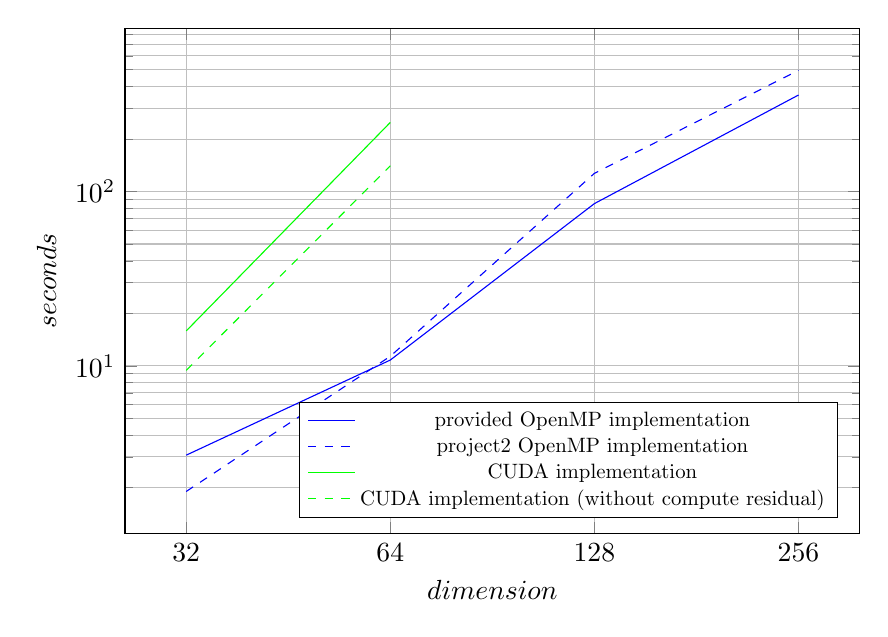
\begin{tikzpicture}
      \begin{axis}[
        width=0.9\textwidth,
        height=8cm,
        xlabel={$dimension$},
        ylabel={$seconds$},
        legend pos=south east,
        legend style={nodes={scale=0.75, transform shape}},
        grid=both,
        xmode=log,
        ymode=log,
        xtick={32,64,128,256},
        xticklabels={32,64,128,256}
      ]

        \addplot[blue,mark=none] coordinates {
          (32,3.07)
          (64,10.79)
          (128,85.26)
          (256,357.93)
        };
        \addlegendentry{provided OpenMP implementation}

        \addplot[blue,dashed,mark=none] coordinates {
          (32,1.90)
          (64,11.34)
          (128,127.18)
          (256,495.89)
        };
        \addlegendentry{project2 OpenMP implementation}

        \addplot[green,mark=none] coordinates {
          (32,15.85)
          (64,249.21)
        };
        \addlegendentry{CUDA implementation}

        \addplot[green,dashed,mark=none] coordinates {
          (32,9.41)
          (64,140.46)
        };
        \addlegendentry{CUDA implementation (without compute residual)}

      \end{axis}
    \end{tikzpicture}
    \caption{Execution Time vs Mesh Dimension}
    \label{fig:execution}
  \end{figure}

  \begin{figure}[H]
    \centering
    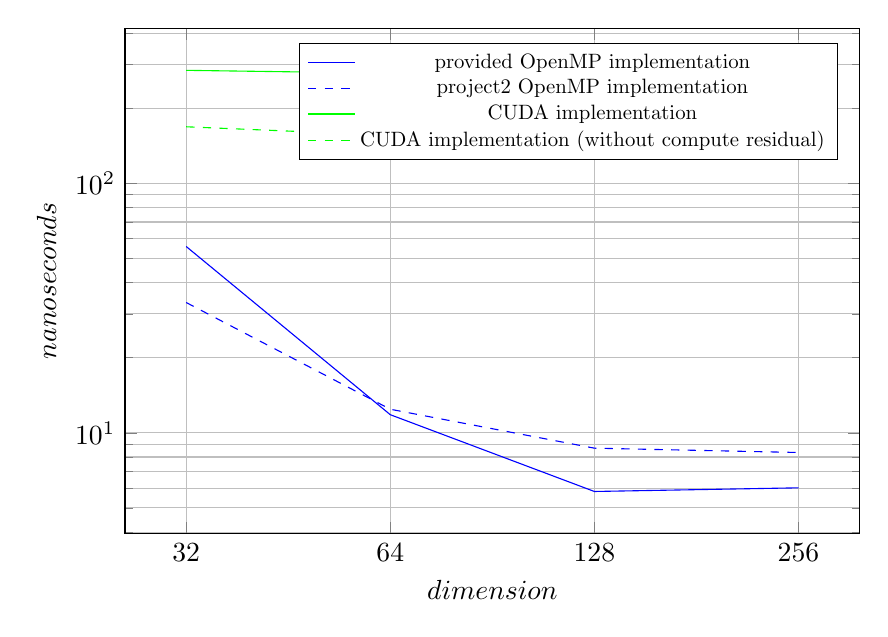
\begin{tikzpicture}
      \begin{axis}[
        width=0.9\textwidth,
        height=8cm,
        xlabel={$dimension$},
        ylabel={$nanoseconds$},
        legend pos=north east,
        legend style={nodes={scale=0.75, transform shape}},
        grid=both,
        xmode=log,
        ymode=log,
        xtick={32,64,128,256},
        xticklabels={32,64,128,256}
      ]

        \addplot[blue,mark=none] coordinates {
          (32,55.81)
          (64,11.82)
          (128,5.82)
          (256,6.02)
        };
        \addlegendentry{provided OpenMP implementation}

        \addplot[blue,dashed,mark=none] coordinates {
          (32,33.28)
          (64,12.43)
          (128,8.68)
          (256,8.34)
        };
        \addlegendentry{project2 OpenMP implementation}

        \addplot[green,mark=none] coordinates {
          (32,283.66)
          (64,276.20)
        };
        \addlegendentry{CUDA implementation}

        \addplot[green,dashed,mark=none] coordinates {
          (32,168.49)
          (64,155.67)
        };
        \addlegendentry{CUDA implementation (without compute residual)}

      \end{axis}
    \end{tikzpicture}
    \caption{Per Cell Time vs Mesh Dimension}
    \label{fig:percell}
  \end{figure}

  The execution time is plotted in Figure~\ref{fig:execution} with both the
  x and y axies using a logarithmic scale since execution time grows linearly
  with mesh size, but the data points have exponential distances between them. 
  Per cell time is also using the same set of scales in 
  Figure~\ref{fig:percell} as it shows the rational nature of the improvements 
  over time.

  Execution time and per cell time is not available for the 128 and 256 mesh
  sizes for the CUDA attempts as the maximum execution time of 30 minutes was
  exceeded, and that information was not recorded.

  An additional set of CUDA runs was included that excluded the 
  \verb|computeResidual| CUDA kernel function during execution, replacing it
  with the original serial implementation. This was done in an attempt to help
  identify possibly where slowdowns were encountered.

  \section{Synthesis}

  References to ``the OpenMP implementation" may refer to either the
  implementation given or the previous \textit{Project 2} implementation.

  As stated in the section 3, the expected time per cell should be about 10
  nanoseconds, and this suggests that the execution time should track (or
  be in the ballpark of) that of the OpenMP implementation, given the
  prior knowledge of the per cell execution time for a comparable mesh size.

  The results show that the implementation of CUDA as outlined in section 2
  was not the most effective. In fact, the execution of mesh sizes of 128 and
  256 never completed within the 30 minute wall time. Based on the 32 and 64
  mesh sizes, the implementation's execution time increases linearly like the
  OpenMP implementation, and extrapolating from there, it's estimated that if
  no wall time was specified, the execution time of the 128 mesh size would
  have been approximately 70 minutes, and the 256 mesh size would be over 17
  hours.

  In an attempt to identify how poor the implementation of CUDA was, a
  variant of the program was compiled and tested where the
  \verb|computeResidual| kernal function was replaced with its serial version.
  The execution time was reduced significantly, indicating that the CUDA
  implementation of the \verb|computeResidual| was significantly slower than
  the serial version.

  Additionally, while the OpenMP implementation exhibited a rational reduction
  of time per cell as shown in Figure~\ref{fig:percell}, the CUDA
  implementation showed no improvement between the 32 and 64 mesh sizes.
  Further, the implementation with the serial execution of 
  \verb|computeResidual| had an improved per cell run time, but also exhibits
  no improvement between the mesh sizes.

  This improvement in overall performance between CUDA implementations, but 
  stagnent improvement between mesh sizes, indicates that the parallelization
  attempt created more bottlenecks than the communication cost between the
  CPU and GPU that was saved, and that there exists further bottlenecks in
  the implementation in other functions.

  The observed peformance of the CUDA code suggests that the memory bandwidth
  is saturated, as with larger and larger meshes, the performance per cell
  remains the same. The granularity may be too large to see actual
  performance increases with larger mesh sizes.

  \section{Conclusion}

  The CUDA implementation as it was implemented is not satisfactory. The
  expectation was similar performance improvements as the OpenMP 
  implementation, but this was not realized. The exact reasons for this were
  not pinpointed, but suggestions on improvement would be to readdress the way 
  that kernel functions access memory or adjust grid sizes used.
  
  Furthermore, a better grasp on the architecture of how CUDA works in context
  of GPU parallelization would aid in addressing these issues.

\end{document}
